\documentclass[12pt]{article}

\usepackage{fontawesome}
\usepackage{hyperref}
\usepackage{xurl}
\usepackage{graphicx}



\hypersetup{
    colorlinks=false,
    pdfborder={0 0 0},
}


\title{Introduction to SQL}
\author{
        Adrianna Holden-Gouveia \\
        Website: \url{https://aholdengouveia.name}\\ 
        \date{\vspace{-5ex}}
        %Email: \href{mailto:admin@aholdengouveia.name}{admin@aholdengouveia.name} \\
        \faLinkedin{: aholdengouveia} \\
        \faGithub {: aholdengouveia} \\
        %\faTwitter {: aholdengouveia} \\
        }

%S\date{\today}


\begin{document}    

\maketitle

%\begin{abstract}
%This is a template for Linux Administration Lab work
%\end{abstract}
%\tableofcontents

\section*{Objectives:}
\begin{itemize}
    \item The objective of this lab is to introduce students to the basic concepts of Structured Query Language (SQL). No prior knowledge of SQL is assumed. Students will gain a basic understanding of SQL through interactive methods utilizing a free online tutorial and other resources.
\end{itemize}
\section*{Instructions}

References, a video, a PowerPoint and some notes are available at my website
\url {https://www.aholdengouveia.name/IntroData/introsql.html}

The tutorial you will be following is here: \url{https://www.khanacademy.org/computing/computer-programming/sql/sql-basics/v/welcome-to-sql} You will be going through of SQL basics.  You should be able to sign up for free, do not pay money. If you run into issues let me know.

\subsection*{Please include answers to the following questions}
    \begin{enumerate}
        \item Have you used SQL before? If yes, for what and how much experience do you have with it?
        \item After completing this, what are your opinions on the difficulty? 
        \item What is one thing you liked about this tutorial? What is one thing you think they could have done better?
        \item If you want to attempt more on Kahn Academy you can, did you try it? If yes, why? If no, why not?
        \item Take screenshots of each completed challenge that you solve, make sure to have a note with your name and the term in the screenshot, screenshot should be focused on the note and answer, not the full desktop.  Any screenshots that don't include the note, or are full desktop, or taken with a camera instead of a screenshot won't count and will earn no points. This is an example of what it should look like:        
 
        \begin{figure}[h!]
            \centerline{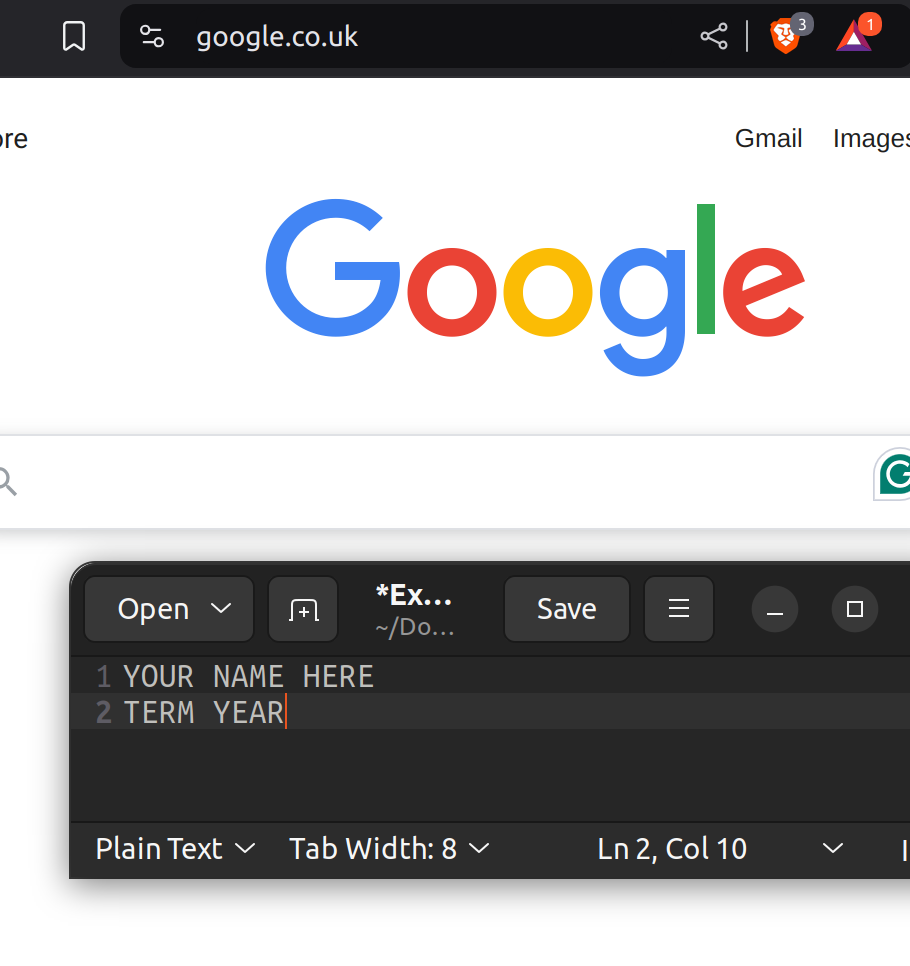
\includegraphics[scale=.2]{ExampleScreenshot.png}}
            \caption{This is an image of what each of your screenshots should look like}

            \end{figure} 
    \end{enumerate}

    \section*{Tutorial Recommendation}
You should find a tutorial that you would recommend to another person that wanted to learn SQL.  The tutorial can be interactive or not.  Videos that you can follow along with count as tutorials for this. You should find at least 3 options for tutorials/videos that you also include here. In your recommendation you should explain why you picked the one you did over the other two including pros and cons of each. 

You may not include any of the links I've shared anywhere on Blackboard or my website in your list, they must be new to you materials and tutorials/videos. 


\section*{Deliverables}
\begin{itemize}
    \item A document containing all requested screenshots
    \item Answers to the above questions
    \item Your tutorial Recommendation.  Review should be at least a paragraph but no more then two pages. 
\end{itemize} 
\end{document}